% Week 3 Lecture Notes: Generative Adversarial Networks
% Generative AI (CS 782/882), Old Dominion University, Fall 2026
% Compile: pdflatex -interaction=nonstopmode week03-notes.tex  (run twice)

% Shared preamble for the Generative AI (CS 782/882, Fall 2026) lecture notes.
% Each weekNN-notes.tex file inlines this block so it compiles on its own.
\documentclass[11pt]{article}
\usepackage[margin=1in]{geometry}
\usepackage[T1]{fontenc}
\usepackage[utf8]{inputenc}
\usepackage{lmodern}
\usepackage{amsmath,amssymb,amsthm,mathtools,bm}
\usepackage{enumitem}
\usepackage{graphicx}
\usepackage{booktabs}
\usepackage{xcolor}
\usepackage{tikz}
\usetikzlibrary{arrows.meta,positioning,calc,shapes}
\usepackage{listings}
\usepackage[colorlinks=true,linkcolor=blue!60!black,urlcolor=blue!60!black,citecolor=blue!60!black]{hyperref}

\newcommand{\E}{\mathbb{E}}
\newcommand{\Var}{\mathrm{Var}}
\newcommand{\KL}{\mathrm{KL}}
\newcommand{\given}{\,\vert\,}
\newcommand{\R}{\mathbb{R}}
\DeclareMathOperator*{\argmax}{arg\,max}
\DeclareMathOperator*{\argmin}{arg\,min}
\newtheorem{theorem}{Theorem}
\newtheorem{lemma}{Lemma}
\newtheorem{definition}{Definition}
\theoremstyle{remark}
\newtheorem*{remark}{Remark}

\lstset{basicstyle=\ttfamily\small,breaklines=true,frame=single,columns=fullflexible}

% ---- Week 3 additions (after the shared preamble) ----
\usetikzlibrary{trees}
\usepackage{array}
\newtheorem{proposition}{Proposition}
\setcounter{tocdepth}{2}
\setlength{\parskip}{4pt}
\setlength{\emergencystretch}{2em}

% Colors for the family tree (from the instructor's GAN-tree.tex)
\definecolor{joint}{HTML}{2B8CBE}
\definecolor{separate}{HTML}{31A354}
\definecolor{cat}{HTML}{444444}

\title{Week 3 Lecture Notes: Generative Adversarial Networks}
\author{Hong Qin, Old Dominion University}
\date{Fall 2026}

\begin{document}
\maketitle
\tableofcontents
\bigskip

\noindent
\textbf{How to read these notes.} Each of the four topics opens with a plain-English summary, then gives the mathematics, then closes with a plain-English payoff. Topics 1 and 2 contain the full derivations from the course tutorial \emph{Principles of GANs: Classical GAN, WGAN, and WGAN-GP}; Topics 3 and 4 are shorter and are meant to be read alongside Foster, \emph{Generative Deep Learning} (2nd ed., 2023), Chapter 4.

% ======================================================================
\section{Topic 1: Generator and Discriminator Objectives}
% ======================================================================

\paragraph{Plain-English summary.}
Module 2 trained a generative model by maximizing a likelihood bound (the ELBO). This module takes a radically different approach: train a generator network by making it compete against a second network, a discriminator, whose job is to tell real data apart from generated data. There is no likelihood, no posterior, and no latent inference. The bet is that the equilibrium of this two-player game produces a generator that fools the discriminator on data drawn from the true distribution. When it works, the samples are noticeably sharper than VAE samples. When it does not work, it fails in spectacular and strange ways; Topic 2 covers those failure modes. This topic sets up the game itself and shows why its equilibrium recovers the data distribution.

\subsection{Background: The Minimax Game}

Generative Adversarial Networks (GANs), introduced by Goodfellow et al.\ (2014), consist of two neural networks trained together in an adversarial setting:
\begin{itemize}
    \item The \textbf{discriminator} $D(x;\theta_d)$ outputs a \emph{probability $D(x)\in[0,1]$} that a sample $x$ comes from the real data distribution $p_{\text{data}}$.
    \item The \textbf{generator} $G(z;\theta_g)$ maps random noise $z\sim p_z(z)$ into synthetic samples, inducing a model distribution $p_g$.
\end{itemize}

\subsubsection*{Why is it a minimax game?}

The interaction between $D$ and $G$ naturally forms a two-player zero-sum game:
\begin{itemize}
    \item The discriminator seeks to \emph{maximize} its ability to distinguish real samples from fake ones. Its payoff is larger when $D(x)$ is close to $1$ for real $x$ and $D(G(z))$ is close to $0$ for generated samples.
    \item The generator seeks to \emph{minimize} this same payoff by producing $G(z)$ such that $D(G(z))$ is close to $1$, making fakes indistinguishable from real.
\end{itemize}

Formally, the value function is
\begin{equation}
    V(D,G) = \mathbb{E}_{x\sim p_{\text{data}}}[\log D(x)]
           + \mathbb{E}_{z\sim p_z}[\log(1-D(G(z)))].
\end{equation}
\emph{The discriminator maximizes $V(D,G)$, while the generator minimizes it}:
\begin{equation}
    \min_G \max_D V(D,G).
\end{equation}

\paragraph{Plain English.}
This is a \emph{minimax game} because one player (the discriminator) is maximizing the score, while the other (the generator) is minimizing the same score. Their goals are directly opposed, much like a counterfeiter vs.\ inspector contest: the inspector wants to catch counterfeits, while the counterfeiter wants to evade detection. At equilibrium, the generator produces realistic samples and the discriminator is reduced to random guessing ($D(x)=0.5$).

\subsubsection*{Why does the second term involve $\log(1-D(G(z)))$?}

The discriminator is trained as a \textbf{binary classifier} with the cross-entropy loss:
\[
\ell(y,D(x)) = y\log D(x) + (1-y)\log(1-D(x)), \qquad y\in\{0,1\}.
\]

Applying this to the GAN setting:

\begin{center}
\renewcommand{\arraystretch}{1.3}
\begin{tabular}{@{}lll@{}}
\toprule
\textbf{Sample type} & \textbf{True label $y$} & \textbf{Contribution to loss} \\
\midrule
Real sample $x\sim p_{\text{data}}$ & $y=1$ & $\log D(x)$ \\
Fake sample $G(z),\, z\sim p_z$ & $y=0$ & $\log (1 - D(G(z)))$ \\
\bottomrule
\end{tabular}
\end{center}

Therefore, the discriminator's expected log-likelihood is exactly
\[
\mathbb{E}_{x\sim p_{\text{data}}}[\log D(x)] + \mathbb{E}_{z\sim p_z}[\log(1-D(G(z)))].
\]

\paragraph{Relation to the Generator.}
The $(1-D(G(z)))$ term arises because fake data are labeled as ``0.''
The generator, in turn, minimizes this same objective, pushing $D(G(z))$ upward so that fakes look real. In practice, to avoid vanishing gradients, $G$ often uses the alternative loss
\[
\mathcal{L}_G = \mathbb{E}_{z\sim p_z}[-\log D(G(z))],
\]
which explicitly encourages $D(G(z))\to 1$.

\subsection{Step-by-Step Derivation for Classical GAN}

\subsubsection{Optimal Discriminator $D^*$}
For fixed $G$, rewrite
\begin{equation}
V(D,G)=\int p_{\text{data}}(x)\log D(x)\,dx+\int p_g(x)\log\big(1-D(x)\big)\,dx.
\end{equation}
Pointwise maximization over $D(x)\in(0,1)$ yields
\[
\frac{\partial}{\partial D(x)}\left[p_{\text{data}}(x)\log D(x)+p_g(x)\log(1-D(x))\right]=0,
\]
so
\begin{equation}
\boxed{D^*(x)=\frac{p_{\text{data}}(x)}{p_{\text{data}}(x)+p_g(x)}.}
\end{equation}

\paragraph{Plain English.}
The best detector at a given $x$ reports the \emph{relative likelihood} of being real vs.\ fake.

\subsubsection{From KL to JSD}
Substitute $D^*$ back into $V$:
\begin{align}
V(D^*,G)
&=\int p_{\text{data}}(x)\log\!\left(\frac{p_{\text{data}}(x)}{p_{\text{data}}(x)+p_g(x)}\right)dx \\
&\quad + \int p_g(x)\log\!\left(\frac{p_g(x)}{p_{\text{data}}(x)+p_g(x)}\right)dx.
\end{align}

Define the \emph{mixture distribution}
\[
m(x) = \tfrac{1}{2}\big(p_{\text{data}} (x)+p_g(x)\big) .
\]

Notice that
\[
\frac{p_{\text{data}}(x)}{p_{\text{data}}(x)+p_g(x)} = \frac{p_{\text{data}}(x)}{2m(x)},\qquad
\frac{p_g(x)}{p_{\text{data}}(x)+p_g(x)} = \frac{p_g(x)}{2m(x)}.
\]

So
\begin{align}
V(D^*,G)
&= \int p_{\text{data}}(x)\Big[\log p_{\text{data}}(x) - \log(2m(x))\Big]\,dx \\
&\quad + \int p_g(x)\Big[\log p_g(x) - \log(2m(x))\Big]\,dx.
\end{align}

Group terms:
\begin{align}
V(D^*,G)
&= \underbrace{\int p_{\text{data}}(x)\log\frac{p_{\text{data}}(x)}{m(x)}dx}_{\mathrm{KL}(p_{\text{data}}\|m)}
+ \underbrace{\int p_g(x)\log\frac{p_g(x)}{m(x)}dx}_{\mathrm{KL}(p_g\|m)} \\
&\quad - 2\log 2.
\end{align}

Thus,
\begin{equation}
\boxed{V(D^*,G) = \mathrm{KL}(p_{\text{data}}\|m) + \mathrm{KL}(p_g\|m) - 2\log 2.}
\end{equation}

\paragraph{Plain English.}
The objective decomposes into two KL divergences: one measuring how far real data is from the mixture, and one measuring how far generated data is from the same mixture.

\subsubsection{From Two KLs to JSD}
The Jensen-Shannon divergence between $p_{\text{data}}$ and $p_g$ is defined as
\begin{equation}
\mathrm{JSD}(p_{\text{data}}\|p_g) = \tfrac{1}{2}\mathrm{KL}(p_{\text{data}}\|m) + \tfrac{1}{2}\mathrm{KL}(p_g\|m),
\end{equation}
with $m=\tfrac{1}{2}(p_{\text{data}}+p_g)$.

Therefore,
\begin{equation}
\mathrm{KL}(p_{\text{data}}\|m) + \mathrm{KL}(p_g\|m) = 2\,\mathrm{JSD}(p_{\text{data}}\|p_g).
\end{equation}

So the generator's true objective simplifies to
\begin{equation}
\boxed{V(D^*,G) = -\log 4 + 2\,\mathrm{JSD}(p_{\text{data}}\|p_g).}
\end{equation}

\paragraph{Plain English.}
Classical GAN training is therefore equivalent to minimizing the Jensen-Shannon divergence between the true and generated distributions.

\subsubsection{KL vs.\ JSD: Relationship}
\begin{itemize}
\item KL divergence $\mathrm{KL}(p\|q)$ is asymmetric and can diverge to $\infty$ if $q(x)=0$ where $p(x)>0$.
\item JSD is a symmetric, smoothed version of KL:
\[
\mathrm{JSD}(p\|q) = \tfrac{1}{2}\mathrm{KL}(p\|m)+\tfrac{1}{2}\mathrm{KL}(q\|m),
\]
where $m=\tfrac12(p+q)$.
\item JSD is always finite and bounded: $0 \le \mathrm{JSD}(p\|q) \le \log 2$.
\end{itemize}

\paragraph{Plain English.}
KL measures divergence in one direction and can blow up if distributions do not overlap. JSD averages two KLs against the mixture, making it symmetric and bounded, but this smoothing also means gradients vanish if $p$ and $q$ are far apart.

\subsubsection{Summary: The Generator's Objective is JSD}
Substituting $D^*$:
\begin{align}
V(D^*,G)
&=\int p_{\text{data}}\log\!\left(\frac{p_{\text{data}}}{p_{\text{data}}+p_g}\right)\,dx
+\int p_g\log\!\left(\frac{p_g}{p_{\text{data}}+p_g}\right)\,dx\\
&=\mathrm{KL}(p_{\text{data}}\|m)+\mathrm{KL}(p_g\|m)-2\log 2\\
&=-\log 4 + 2\,\mathrm{JSD}(p_{\text{data}}\|p_g),
\end{align}
where $m=\tfrac12(p_{\text{data}}+p_g)$.

\paragraph{Plain English.}
With an optimal discriminator, classical GAN effectively minimizes the \emph{Jensen-Shannon divergence (JSD)} between real and model distributions.

\subsubsection{Equilibrium}
Since $\mathrm{JSD}\ge 0$ and is $0$ iff $p_g=p_{\text{data}}$, the global optimum is
\[
p_g=p_{\text{data}},\qquad D^*(x)=\tfrac12,\qquad V(D^*,G)=-\log 4.
\]

\subsection{Training Process for the Classical GAN}

Training GANs involves solving the minimax problem
\[
\min_G \max_D V(D,G),
\]
where the discriminator tries to maximize $V(D,G)$ and the generator tries to minimize it. In practice, this is implemented through alternating gradient-based updates.

\begin{enumerate}
\item \textbf{Sample minibatches:}
Draw real data $\{x^{(i)}\}\sim p_{\text{data}}$ and noise vectors $\{z^{(i)}\}\sim p_z$.
These provide the positive (real) and negative (fake) examples needed for training $D$.

\item \textbf{Update the discriminator (maximize):}
\[
\mathcal{L}_D=\mathbb{E}_{x\sim p_{\text{data}}}[\log D(x)] + \mathbb{E}_{z\sim p_z}[\log(1-D(G(z)))].
\]
This loss is the log-likelihood of correctly classifying both real and fake samples.
In practice, we \emph{maximize} $\mathcal{L}_D$ by performing gradient ascent on $D$'s parameters:
\[
\theta_d \leftarrow \theta_d + \eta \nabla_{\theta_d} \mathcal{L}_D,
\]
where $\eta$ is the learning rate.
This moves $D$ toward higher accuracy as a binary classifier.

\item \textbf{Update the generator (minimize):}

If we used the original minimax form, the generator would minimize
\[
\mathbb{E}_{z\sim p_z}[\log(1-D(G(z)))].
\]
However, this saturates when $D$ is strong.

To provide stronger gradients, we instead minimize the \emph{non-saturating loss}:
\[
\mathcal{L}_G = \mathbb{E}_{z\sim p_z}[-\log D(G(z))],
\]
which is equivalent to maximizing $\mathbb{E}_{z\sim p_z}[\log D(G(z))]$.

In practice, we perform gradient descent on $G$'s parameters:
\[
\theta_g \leftarrow \theta_g - \eta \nabla_{\theta_g} \mathcal{L}_G.
\]
This encourages $D(G(z))$ to become large, i.e.\ for $D$ to classify generated samples as ``real.''
\end{enumerate}

\paragraph{How min and max are achieved.}
\begin{itemize}
    \item The \textbf{maximization step} for $D$ is achieved by updating its parameters to increase $\mathcal{L}_D$ (gradient ascent). Intuitively, $D$ improves at separating real from fake.
    \item The \textbf{minimization step} for $G$ is achieved by updating its parameters to decrease $\mathcal{L}_G$ (gradient descent). Intuitively, $G$ improves at producing samples that fool $D$.
    \item Alternating these steps approximates the game $\min_G \max_D V(D,G)$. When training is balanced, $D$ stays near its optimal solution given $G$, and $G$ steadily reduces the divergence between $p_g$ and $p_{\text{data}}$.
\end{itemize}

\paragraph{Plain English.}
Training GANs is like teaching two opponents in a game:
\begin{itemize}
    \item First, train the \emph{detector} ($D$) to better spot real vs.\ fake by rewarding correct guesses.
    \item Then, train the \emph{forger} ($G$) to make fakes more convincing by rewarding it when the detector is fooled.
\end{itemize}
The ``max'' step is $D$ becoming a better cop, and the ``min'' step is $G$ becoming a better counterfeiter. Repeating this back-and-forth process drives the system toward equilibrium.

\subsection{Generator Loss Functions: Minimax vs.~Non-Saturating}

In the original GAN framework (Goodfellow et al., 2014), the generator
minimizes the following \emph{minimax} loss:
\begin{equation}
\label{eq:minimax}
\mathcal{L}^{\text{minimax}}_G(\theta)
= \mathbb{E}_{z\sim p_z}\Big[\log\!\big(1-D_\phi(G_\theta(z))\big)\Big],
\end{equation}
where $D_\phi(x)=\sigma(a_\phi(x))$ is the discriminator (sigmoid of pre-activation $a_\phi(x)$)
and $G_\theta(z)$ is the generator.

\subsubsection{Gradient of the Minimax Generator Loss}

Differentiating \eqref{eq:minimax} with respect to $\theta$:
\begin{align}
\nabla_\theta \log(1-D)
&= -\frac{1}{1-\sigma(a)}\,\sigma'(a)\,\nabla_\theta a, \\
&= -\sigma(a)\,\nabla_\theta a,
\end{align}
since $\sigma'(a)=\sigma(a)(1-\sigma(a))$.
Therefore,
\begin{equation}
\label{eq:minimax_grad}
\nabla_\theta \mathcal{L}^{\text{minimax}}_G
= \mathbb{E}_{z}\Big[-\,\sigma\!\big(a(G_\theta(z))\big)\,\nabla_\theta a(G_\theta(z))\Big].
\end{equation}

\paragraph{Saturation.}
When the discriminator is strong at distinguishing fakes, $D(G_\theta(z))\approx 0$,
so $\sigma(a)\approx 0$. The prefactor in \eqref{eq:minimax_grad} vanishes, leading
to very weak gradients for the generator.

\subsubsection{Gradient of the Non-Saturating Generator Loss}

To alleviate saturation, Goodfellow et al.\ (2014) proposed the
\emph{non-saturating} surrogate:
\begin{equation}
\label{eq:ns_loss}
\mathcal{L}^{\text{NS}}_G(\theta)
= \mathbb{E}_{z\sim p_z}\Big[-\log D_\phi(G_\theta(z))\Big]
= \mathbb{E}_{z}\Big[-\log \sigma(a)\Big].
\end{equation}
Differentiating,
\begin{align}
\nabla_\theta \big[-\log \sigma(a)\big]
&= -\frac{\sigma'(a)}{\sigma(a)}\,\nabla_\theta a, \\
&= -(1-\sigma(a))\,\nabla_\theta a.
\end{align}
Hence,
\begin{equation}
\label{eq:ns_grad}
\nabla_\theta \mathcal{L}^{\text{NS}}_G
= \mathbb{E}_{z}\Big[-\big(1-\sigma(a(G_\theta(z)))\big)\,\nabla_\theta a(G_\theta(z))\Big].
\end{equation}

\paragraph{Contrast with minimax.}
\begin{itemize}
  \item Minimax gradient factor: $-\sigma(a)$.
  \item Non-saturating gradient factor: $-(1-\sigma(a))$.
\end{itemize}
When $D(G_\theta(z))\approx 0$, the minimax factor $\sigma(a)\approx 0$,
but the non-saturating factor $(1-\sigma(a))\approx 1$, so the generator
receives strong gradients.

\subsubsection{Label-Flipping View}

Discriminator training minimizes the binary cross-entropy
\begin{equation}
\mathcal{L}_D
= -\mathbb{E}_{x\sim p_{\text{data}}}\log D(x)
 -\mathbb{E}_{z\sim p_z}\log\!\big(1-D(G(z))\big).
\end{equation}
The minimax generator uses the same second term,
while the non-saturating generator ``flips'' the fake label to~1:
\begin{equation}
\mathcal{L}^{\text{NS}}_G = -\mathbb{E}_{z}\log D(G(z)).
\end{equation}

\subsubsection{Shared Equilibrium}

Both objectives share the same fixed point. With the optimal discriminator
\[
D^*(x)=\frac{p_{\text{data}}(x)}{p_{\text{data}}(x)+p_g(x)},
\]
the minimax reduces to $-\log 4 + 2\,\mathrm{JSD}(p_{\text{data}}\|p_g)$,
minimized at $p_g=p_{\text{data}}$. For the non-saturating case,
when $p_g=p_{\text{data}}$, one obtains $D^*(x)=\tfrac12$ for all~$x$,
hence $\mathcal{L}^{\text{NS}}_G=-\log\tfrac12$ (a constant),
so the gradient vanishes and equilibrium is achieved at the same solution.

\subsubsection{Magnitude Comparison}

For $s=D(G_\theta(z))=\sigma(a)\in(0,1)$ and fixed $\nabla_\theta a$:
\begin{align}
g_{\text{MM}}(z) &= -s\,\nabla_\theta a, \\
g_{\text{NS}}(z) &= -(1-s)\,\nabla_\theta a.
\end{align}
If $s\le \tfrac{1}{2}$, then $|g_{\text{NS}}(z)| \ge |g_{\text{MM}}(z)|$,
with equality only at $s=\tfrac12$. As $s\to 0$, the minimax gradient vanishes,
while the non-saturating gradient maintains full strength.

\paragraph{Summary.}
\begin{itemize}
  \item \textbf{Minimax:} gradient $\propto -D(G(z))$; vanishes when $D(G(z))\approx 0$.
  \item \textbf{Non-saturating:} gradient $\propto -(1-D(G(z)))$; remains strong
        when $D(G(z))\approx 0$.
  \item Both converge to the same equilibrium $p_g=p_{\text{data}}$.
\end{itemize}

\subsection{Why the Generator/Discriminator Use Noise}
Noise $z$ drives diversity in $G(z)$ and creates fake samples for $D$ to learn from. Without noise, $G$ collapses to a constant and $D$ would trivially predict ``real'' (no learning signal).

\paragraph{Plain-English payoff.}
The whole of Topic 1 can be compressed into three sentences. A GAN replaces the likelihood with a game: the discriminator is an ordinary binary classifier, and the generator is trained to make that classifier fail. If the discriminator is allowed to be optimal, the game is secretly minimizing the Jensen-Shannon divergence between the data and the model, so the unique winner is $p_g=p_{\text{data}}$. The theory holds only \emph{if} training reaches that saddle point, and Topic 2 is about why, in practice, it often does not.

\paragraph{Further reading.}\begingroup\sloppy
I.\ Goodfellow et al., ``Generative Adversarial Networks,'' NeurIPS 2014, arXiv:1406.2661 (Sections 3 and 4 for the saddle-point setup and the convergence argument). I.\ Goodfellow, ``NIPS 2016 Tutorial: Generative Adversarial Networks,'' arXiv:1701.00160. Foster (2023), Chapter 4, sections ``Introduction to GANs'' and ``Your First GAN.''
\endgroup

% ======================================================================
\section{Topic 2: Adversarial Training Dynamics and Instability}
% ======================================================================

\paragraph{Plain-English summary.}
Topic 1 showed that, in theory, the GAN equilibrium recovers the data distribution. The catch is ``in theory.'' Training a minimax game is genuinely hard: it can oscillate forever, collapse to a single output mode, produce losses that tell you nothing useful, or be devastatingly sensitive to hyperparameters. This topic first names the four canonical failure modes, then explains the mathematical reason GAN training is intrinsically harder than VAE training (the Jensen-Shannon divergence goes flat when the two distributions do not overlap), and finally presents the Wasserstein GAN family, which is the fix the community converged on.

\subsection{Four Named Failure Modes}

Foster (Chapter 4, ``GAN Challenges'') groups GAN training pathologies into four:
\begin{enumerate}
    \item \textbf{Oscillating loss.} The discriminator and generator losses bounce around indefinitely instead of converging. The game has no monotone progress metric.
    \item \textbf{Mode collapse.} The generator finds one output (or a small set of outputs) that fools the discriminator and gets stuck producing only that. The other modes of the data distribution disappear from the samples.
    \item \textbf{Uninformative loss.} The discriminator and generator losses are not a useful signal of sample quality. A falling discriminator loss does not mean the samples are improving; a falling generator loss does not mean the generator is winning.
    \item \textbf{Hyperparameter sensitivity.} Small changes to the learning rate, batch size, or architecture can turn a working GAN into a broken one. There is no robust autopilot configuration.
\end{enumerate}
You will see at least one of these in any non-trivial GAN training run. Recognizing them by name is half of the diagnosis; the mathematics below explains where the first three come from.

\subsection{Weakness of the Classical GAN}
The classical GAN uses JSD between $p_{\text{data}}$ and $p_g$.
\begin{itemize}
\item When $p_{\text{data}}$ and $p_g$ have little or no support overlap (common in high-$d$), the JSD becomes constant.
\item Constant JSD $\Rightarrow$ vanishing gradients for $G$; training stalls/oscillates.
\end{itemize}

\paragraph{Plain English.}
In high dimensions, real and fake can be far apart. JSD then goes flat, so $G$ receives no useful direction to move.

\paragraph{Why supports rarely overlap early in training.}
Real images (or any structured data) live near a low-dimensional manifold inside a very high-dimensional space, and the generator's early outputs are essentially noise. Two such sets almost never overlap, so $\mathrm{JSD}(p_{\text{data}}\|p_g)$ sits at its maximum value $\log 2$ regardless of how far apart the distributions are. That constant has zero gradient with respect to the generator parameters. This is the deep reason a discriminator can ``get too good too fast'' and break training: an optimal discriminator is exactly the one that exposes the flat JSD.

% ==========================================================
\subsection{Wasserstein GAN (WGAN)}

\subsubsection{From Optimal Transport to a Learnable Objective}
The Wasserstein-1 (Earth Mover) distance between two distributions $p$ and $q$ on $\mathcal{X}\subset\mathbb{R}^d$ is
\begin{equation}
W_1(p,q)=\inf_{\gamma\in\Pi(p,q)} \ \mathbb{E}_{(x,y)\sim\gamma}\big[\|x-y\|_2\big],
\label{eq:primal}
\end{equation}
where $\Pi(p,q)$ are couplings with marginals $p$ and $q$.

\paragraph{Plain English.}
Imagine all ways to ``relabel'' (or transport) probability mass from $p$ to $q$; $W_1$ is the \emph{least} average distance you must move that mass.

\subsubsection{Kantorovich-Rubinstein Duality (Critic View)}
Define $\mathcal{F}_1=\{f:\mathcal{X}\to\mathbb{R} \mid \|f\|_{\mathrm{Lip}}\le 1\}$, the set of all $1$-Lipschitz functions. The dual form is
\begin{equation}
W_1(p,q)=\sup_{f\in\mathcal{F}_1}\left(\mathbb{E}_{x\sim p}[f(x)]-\mathbb{E}_{y\sim q}[f(y)]\right).
\label{eq:dual}
\end{equation}

\paragraph{What does ``supremum'' mean here?}
$\sup$ = \emph{least upper bound}. We scan over all $1$-Lipschitz $f$ and pick the largest possible expectation gap. This ``best lens'' $f^*$ is called a \emph{Kantorovich potential}.

\paragraph{Plain English.}
Instead of explicitly moving mass (primal view), we score samples with a function whose slope is at most $1$. The best such scorer separates real from fake as much as allowed; that max separation equals the transport cost.

\subsubsection{Turning the Dual into a GAN Objective}
Let $p=p_{\text{data}}$ and $q=p_g$ (the generator's distribution). Parameterize $f$ by a neural network $f_w$ (the \emph{critic}) and enforce $\|f_w\|_{\mathrm{Lip}}\le 1$. Then:
\begin{align}
\max_{w \ : \ \|f_w\|_{\mathrm{Lip}}\le 1} \quad
& \mathbb{E}_{x\sim p_{\text{data}}}[f_w(x)] \;-\; \mathbb{E}_{z\sim p_z}[f_w(G_\theta(z))],
\label{eq:wgan-critic}\\
\min_{\theta} \quad
& -\,\mathbb{E}_{z\sim p_z}[f_w(G_\theta(z))].
\label{eq:wgan-gen}
\end{align}

If the inner maximization reaches the supremum in \eqref{eq:dual}, the value equals $W_1(p_{\text{data}},p_g)$, and the generator step \eqref{eq:wgan-gen} \emph{minimizes the Wasserstein distance}.

\paragraph{Plain English.}
We train a critic to give higher scores to real data than to generated data, with a slope cap. Then we train $G$ to increase its scores, which \emph{shrinks} the Earth Mover distance to real data.

\subsubsection{Empirical (Finite-Sample) Objective}
Expectations are approximated by minibatch averages:
\begin{align}
\widehat{\mathcal{L}}_{\text{critic}}
&= \frac{1}{m}\sum_{i=1}^m f_w(x^{(i)}) \;-\; \frac{1}{m}\sum_{i=1}^m f_w(G_\theta(z^{(i)})),
\label{eq:emp-critic}\\
\widehat{\mathcal{L}}_{G}
&= - \frac{1}{m}\sum_{i=1}^m f_w(G_\theta(z^{(i)})).
\label{eq:emp-gen}
\end{align}
We \emph{ascend} $w$ on \eqref{eq:emp-critic} (critic maximization) and \emph{descend} $\theta$ on \eqref{eq:emp-gen} (generator minimization), while enforcing the Lipschitz constraint on $f_w$.

\paragraph{Plain English.}
In practice we just take averages over a minibatch and do standard gradient steps, exactly like everyday deep learning.

\subsubsection{Why No Sigmoid? Scores vs.\ Probabilities}
In classical GANs, $D$ outputs a probability via a sigmoid and is trained with cross-entropy. In WGAN, the critic $f_w$ outputs a \emph{real score} with no sigmoid and is trained to \emph{maximize a gap}. The score scale is meaningful because it estimates $W_1$.

\paragraph{Plain English.}
Do not squeeze the critic through a probability. Let it be a linear ``score''; that is what connects directly to transport distance.

\subsubsection{Gradients for the Generator and Non-vanishing Signal}
By the chain rule,
\begin{equation}
\nabla_\theta \widehat{\mathcal{L}}_{G}
= - \frac{1}{m}\sum_{i=1}^m \Big[\nabla_x f_w(x)\big|_{x=G_\theta(z^{(i)})}\Big]\;\nabla_\theta G_\theta(z^{(i)}).
\label{eq:gen-grad}
\end{equation}
If $f_w$ is $1$-Lipschitz, then (by Rademacher's theorem) $\nabla_x f_w$ exists a.e.\ and $\|\nabla_x f_w(x)\|_2\le 1$. Hence, the generator receives a controlled, \emph{non-saturating} gradient even when $p_{\text{data}}$ and $p_g$ are disjoint.

\paragraph{Plain English.}
The critic's slope is bounded, so $G$ always gets a usable training signal pointing it toward real data, with no flatlines like with JSD.

\subsubsection{How the Max and Min Are Actually Achieved}
\begin{enumerate}
\item \textbf{Critic (inner max).} Take $n_{\text{critic}}$ gradient-ascent steps on \eqref{eq:emp-critic} \emph{while} enforcing $\|f_w\|_{\mathrm{Lip}}\le 1$. The goal is to approach the supremum (or a good approximation) for the current generator.
\item \textbf{Generator (outer min).} Take one gradient-descent step on \eqref{eq:emp-gen} using the current critic. This moves $p_g$ along directions that \emph{reduce} the critic gap, i.e., reduce $W_1$.
\end{enumerate}

\paragraph{Plain English.}
Let the critic sharpen its separation a few times; then let the generator respond once. Repeat. That is how we approximate the $\max$ inside $\min$.

\subsubsection{Enforcing the $1$-Lipschitz Constraint}
Two standard approaches:
\begin{itemize}
\item \textbf{Weight clipping (WGAN).} After each critic update, clip each weight into $[-c,c]$. Simple but can cripple capacity and cause optimization issues.
\item \textbf{Gradient penalty (WGAN-GP).} Add
\[
\lambda\,\mathbb{E}_{\hat{x}}\!\left(\|\nabla_{\hat{x}} f_w(\hat{x})\|_2-1\right)^2,
\quad \hat{x}=\epsilon x+(1-\epsilon)G_\theta(z),\ \epsilon\sim U[0,1],
\]
to softly enforce $\|\nabla f_w\|\approx 1$ where it matters.
\end{itemize}

\paragraph{Plain English.}
Either keep the critic weights in a box (clipping) or teach its \emph{slope} to be $1$ along the data manifold (penalty). The latter is usually smoother.

\subsubsection{Why the WGAN Objective is ``Meaningful''}
If training is balanced (critic near its inner optimum):
\[
\widehat{\mathcal{L}}_{\text{critic}}\ \approx\ W_1(p_{\text{data}},p_g),
\quad
\widehat{\mathcal{L}}_{G}\ \approx\ -W_1(p_{\text{data}},p_g).
\]
As samples improve, $W_1$ decreases \emph{monotonically}, so the losses correlate with visual quality.

\paragraph{Plain English.}
Unlike JSD loss, the WGAN critic loss goes down steadily as samples get better. You can \emph{trust} it as a progress meter.

\subsubsection*{Tiny 1D sanity check (supremum revisited)}
For $p=\delta_0$ and $q=\delta_1$,
\[
W_1(p,q)=\sup_{\|f\|_{\text{Lip}}\le 1}\big(f(0)-f(1)\big)=1,
\]
achieved by $f(x)=-x$. The generator gradient \eqref{eq:gen-grad} points $G(z)$ toward $0$ (the real mass location), giving a non-zero, stable direction.

\paragraph{Plain English.}
The best critic is the line with slope $-1$. Its gradient literally points fake samples toward the real location, exactly what we want.

% ==========================================================
\subsection{WGAN with Gradient Penalty (WGAN-GP)}

\subsubsection{Motivation}
Weight clipping enforces the $1$-Lipschitz constraint crudely by truncating parameters $w\!\in\![-c,c]$, which (i) limits critic capacity, (ii) creates optimization pathologies (flat or exploding regions), and (iii) makes performance sensitive to $c$.
\textbf{WGAN-GP} replaces clipping with a \emph{soft constraint} that penalizes deviations of the critic's input-gradient norm from $1$ along paths that connect real and generated samples.

\paragraph{Plain English.}
Instead of squeezing all critic weights into a tiny box, we encourage the critic to have \emph{unit slope} where it matters. This tends to produce a stronger, smoother critic and more stable training.

\subsubsection{Theoretical Basis: Lipschitzness and the Unit-Gradient Property}
Let $f^\star$ be an optimal Kantorovich potential in the dual of $W_1$. For a $1$-Lipschitz function $f$:
\[
\|\nabla_x f(x)\|_2 \le 1 \quad \text{a.e. (Rademacher's theorem).}
\]
Under mild regularity, along directions used by the optimal transport plan between $p_{\text{data}}$ and $p_g$, the optimal potential tends to be \emph{saturated}, i.e., $\|\nabla_x f^\star(x)\|_2 = 1$ almost everywhere on those paths.

\paragraph{Plain English.}
A $1$-Lipschitz function cannot be steeper than slope $1$. The best critic (for Earth Mover distance) typically pushes right up to that limit along the routes where probability mass moves from fake to real; hence ``unit slope'' along those paths.

\subsubsection{Gradient Penalty: Construction and Intuition}
Sample real $x\!\sim\!p_{\text{data}}$, fake $\tilde{x}\!=\!G_\theta(z)$ with $z\!\sim\!p_z$, draw $\epsilon\!\sim\!\mathrm{Uniform}(0,1)$, and form a random point \emph{on the line} between them:
\[
\hat{x} \;=\; \epsilon\,x + (1-\epsilon)\,\tilde{x}.
\]
Define the critic (maximization) objective with a \emph{two-sided} penalty:
\begin{equation}
\max_{w}\quad
\mathbb{E}_{x}[f_w(x)] - \mathbb{E}_{z}[f_w(G_\theta(z))]
\;-\;
\lambda\,\mathbb{E}_{\hat{x}}
\Big(\,\|\nabla_{\hat{x}} f_w(\hat{x})\|_2 - 1\,\Big)^2,
\label{eq:wgan-gp-critic}
\end{equation}
with $\lambda>0$ (often $\lambda\!=\!10$). The generator objective is unchanged:
\[
\min_{\theta}\quad \mathcal{L}_G \;=\; -\,\mathbb{E}_{z}[\,f_w(G_\theta(z))\,].
\]

\paragraph{Why penalize $\|\nabla f\|_2 \!\approx\! 1$?}
Since an optimal $1$-Lipschitz critic saturates to unit slope \emph{along the transport paths}, nudging $\|\nabla f\|$ toward $1$ on random line segments between real and fake encourages the critic toward the right function class without crippling capacity.

\subsubsection{Where to Sample $\hat{x}$ (and Variants)}
\begin{itemize}
\item \textbf{Between real and fake (standard WGAN-GP).} $\hat{x}=\epsilon x+(1-\epsilon)\tilde{x}$. Targets the regions that connect current fake samples to the data manifold.
\item \textbf{Around real only (R1).} Penalize $\|\nabla_x f(x)\|^2$ at real $x$; useful when focusing smoothness on the data manifold.
\item \textbf{Around fake only (R2).} Penalize at generated points; can complement certain generators.
\item \textbf{Local noise around data (DRAGAN-style).} Perturb real $x$ with small noise and penalize there; encourages stability near data support.
\end{itemize}

\paragraph{Plain English.}
You can teach the critic to have unit slope on (i) the straight lines between real and fake (most common), (ii) right on real data, (iii) on fake data, or (iv) in a noisy band around real data. The standard choice works well in practice.

\subsubsection{Step-by-Step Training with Implementation Details}
\begin{enumerate}
\item \textbf{Critic update (repeat $n_{\text{critic}}$ times, e.g., $5$):}
\begin{enumerate}
\item Sample minibatch $\{x^{(i)}\}_{i=1}^m\sim p_{\text{data}}$, $\{z^{(i)}\}_{i=1}^m\sim p_z$, and form $\tilde{x}^{(i)}=G_\theta(z^{(i)})$.
\item Draw $\epsilon^{(i)}\sim U[0,1]$ and set $\hat{x}^{(i)}=\epsilon^{(i)}x^{(i)}+(1-\epsilon^{(i)})\tilde{x}^{(i)}$.
\item Compute critic scores $f_w(x^{(i)}),\,f_w(\tilde{x}^{(i)}),\,f_w(\hat{x}^{(i)})$.
\item Compute per-sample gradients $g^{(i)}=\nabla_{\hat{x}^{(i)}} f_w(\hat{x}^{(i)})$ via autodiff \emph{w.r.t.\ the input}; then norms $\|g^{(i)}\|_2$.
\item Form the loss (we \emph{maximize} in $w$; in code, typically \emph{minimize the negative}):
\[
\mathcal{L}_{\text{critic}}
=
\frac{1}{m}\!\sum_{i=1}^m f_w(x^{(i)})
- \frac{1}{m}\!\sum_{i=1}^m f_w(\tilde{x}^{(i)})
- \lambda\,\frac{1}{m}\!\sum_{i=1}^m \big(\|g^{(i)}\|_2-1\big)^2.
\]
\item \textbf{Important practice:}
\begin{itemize}
\item Detach $\tilde{x}^{(i)}$ from $G$ when updating the critic (no gradients to $\theta$).
\item When computing $g^{(i)}$, enable higher-order grads (e.g., \texttt{create\_graph=True}) so the penalty can backprop to $w$.
\end{itemize}
\item Take a gradient-ascent step on $w$ (or descent on $-\mathcal{L}_{\text{critic}}$).
\end{enumerate}

\item \textbf{Generator update (once):}
\begin{enumerate}
\item Sample $\{z^{(i)}\}_{i=1}^m\sim p_z$; compute $\tilde{x}^{(i)}=G_\theta(z^{(i)})$.
\item Evaluate critic $f_w(\tilde{x}^{(i)})$ (no penalty here).
\item Minimize
\[
\mathcal{L}_G \;=\; -\frac{1}{m}\sum_{i=1}^m f_w(\tilde{x}^{(i)}),
\]
via gradient descent on $\theta$.
\end{enumerate}
\end{enumerate}

\paragraph{Plain English.}
For the critic: look at real and fake, then also at points in between; make your score higher on real than fake, \emph{and} keep your slope around $1$ on those in-between points. For the generator: change your outputs so the critic gives them higher scores.

\subsubsection{One-Sided vs.\ Two-Sided Penalties}
The standard WGAN-GP uses a \emph{two-sided} penalty $(\|\nabla f\|-1)^2$, encouraging gradients to be close to $1$ from above or below. A \emph{one-sided} version penalizes only when $\|\nabla f\|_2>1$:
\[
\lambda\,\mathbb{E}_{\hat{x}}\!\big[\max(0,\|\nabla_{\hat{x}} f_w(\hat{x})\|_2 - 1)\big]^2,
\]
which more directly enforces the Lipschitz \emph{upper} bound. Empirically, two-sided often trains slightly smoother.

\subsubsection{Why This Improves Gradients to $G$}
Using the chain rule, the generator gradient is
\[
\nabla_\theta \mathcal{L}_G
= -\,\mathbb{E}_{z}\!\left[\nabla_x f_w(x)\big|_{x=G_\theta(z)} \;\nabla_\theta G_\theta(z)\right].
\]
With the GP, $\|\nabla_x f_w\|_2$ is well-behaved (near $1$ along the relevant paths), so $G$ receives a stable, informative signal even when $p_g$ and $p_{\text{data}}$ are initially far apart (disjoint supports).

\paragraph{Plain English.}
The critic's slope is kept in a healthy range; $G$ always gets a clear direction to move its samples closer to the data.

\subsubsection{Hyperparameters and Practical Tips}
\begin{itemize}
\item \textbf{Penalty weight $\lambda$:} commonly $10$; too small $\Rightarrow$ poor constraint; too large $\Rightarrow$ critic underfits the gap.
\item \textbf{$n_{\text{critic}}$:} $3$ to $10$ critic steps per $G$ step (often $5$). More steps let the critic approach its inner optimum.
\item \textbf{Batch norm:} Avoid BN in the critic (its batch coupling can conflict with gradient computations). Use LayerNorm/InstanceNorm or none.
\item \textbf{Per-sample gradient norm:} Compute $\|\nabla f(\hat{x}^{(i)})\|$ \emph{per example} and average; do not average gradients before taking the norm.
\item \textbf{Detach policy:} When updating $w$, treat $G$ outputs as constants (no gradient to $\theta$); when updating $\theta$, do not backprop the GP term.
\item \textbf{Optimizers:} Adam or RMSProp with conservative settings (e.g., Adam $\beta_1\!\in[0.0,0.5]$, $\beta_2\!=\!0.9$).
\end{itemize}

\subsubsection{Advantages and Weaknesses of WGAN-GP}
\paragraph{Advantages.}
\begin{itemize}
\item Stronger, smoother critics than clipping; more stable training.
\item Loss correlates with quality (monotone $W_1$ proxy); fewer vanishing gradients.
\item Often reduces mode collapse relative to classical GANs.
\end{itemize}

\paragraph{Weaknesses.}
\begin{itemize}
\item Extra compute: must backprop through $\nabla_{\hat{x}} f$ each critic step.
\item Sensitivity to $\lambda$ and to where/how $\hat{x}$ is sampled.
\item Only \emph{encourages} $1$-Lipschitzness (not a hard guarantee); bias in $W_1$ estimate is possible.
\item Architectural caveats (avoid BatchNorm in critic; watch activation saturation).
\end{itemize}

\subsubsection*{1D Intuition Check (revisited)}
Let $p=\delta_0$, $q=\delta_1$, and draw $\hat{x}=\epsilon\cdot 0 + (1-\epsilon)\cdot 1 = 1-\epsilon \in [0,1]$.
The optimal critic is $f^\star(x)=-x$ with slope $-1$ everywhere, hence $\|\nabla f^\star(\hat{x})\|_2=1$ along the entire segment.
The GP term is zero when the critic matches this behavior.

\paragraph{Plain English.}
If real mass is at $0$ and fake at $1$, the best critic is a straight line of slope $-1$ between them. The gradient penalty pushes the learned critic toward that shape.

% ==========================================================
\subsection{Comparisons}

\begin{center}
\renewcommand{\arraystretch}{1.15}
\begin{tabular}{@{}p{3.2cm}p{4.6cm}p{6.6cm}@{}}
\toprule
\textbf{Method} & \textbf{Core Idea} & \textbf{Pros / Cons}\\
\midrule
Classical GAN (JSD) &
Minimax on $\log D$ vs.\ $\log(1-D)$; minimizes JSD at optimum. &
\textbf{+} Simple; widely used.\newline
\textbf{$-$} JSD flat when supports disjoint $\Rightarrow$ vanishing gradients; unstable dynamics.\\
\midrule
WGAN (Clipping) &
Maximizes critic gap under $1$-Lipschitz (via weight clipping); minimizes $W_1$. &
\textbf{+} Meaningful loss; non-vanishing gradients; better stability.\newline
\textbf{$-$} Clipping harms capacity; sensitive to $c$, $n_{\text{critic}}$.\\
\midrule
WGAN-GP &
Enforce Lipschitz via gradient penalty along lines between real/fake. &
\textbf{+} Stronger critic; smoother training; good correlation with quality.\newline
\textbf{$-$} Extra compute; hyperparameter sensitivity; only approximate Lipschitz.\\
\bottomrule
\end{tabular}
\end{center}

\subsubsection{Practical Notes (All Methods)}
\begin{itemize}
\item Use the ``non-saturating'' generator loss for classical GANs to avoid vanishing gradients.
\item In WGAN/WGAN-GP, train the critic multiple steps per generator step ($n_{\text{critic}}\in[3,10]$ commonly).
\item Avoid batch normalization in the critic; consider alternatives or none.
\item Spectral normalization is another Lipschitz control technique (alternative to GP/clipping).
\end{itemize}

\paragraph{Plain-English payoff.}
Three practical consequences follow from switching to the Wasserstein objective. First, the critic can be trained close to optimality without killing the generator's gradient, which is the opposite of the JSD case; five critic updates per generator update is the standard schedule. Second, the critic loss becomes a meaningful progress meter that tracks sample quality, so you can monitor training from the loss curve. Third, mode collapse becomes much rarer (not impossible, but qualitatively less frequent). Among the four failure modes, oscillating loss and uninformative loss are the ones you can spot from a loss plot alone; mode collapse and hyperparameter sensitivity usually require looking at sample grids across runs.

\paragraph{Further reading.}\begingroup\sloppy
M.\ Arjovsky, S.\ Chintala, L.\ Bottou, ``Wasserstein GAN,'' ICML 2017, arXiv:1701.07875. I.\ Gulrajani et al., ``Improved Training of Wasserstein GANs,'' NeurIPS 2017, arXiv:1704.00028. T.\ Salimans et al., ``Improved Techniques for Training GANs,'' NeurIPS 2016, arXiv:1606.03498. L.\ Mescheder, A.\ Geiger, S.\ Nowozin, ``Which Training Methods for GANs do actually Converge?'' ICML 2018, arXiv:1801.04406. Foster (2023), Chapter 4, sections ``GAN Challenges,'' ``Wasserstein GAN,'' and ``WGAN-GP.''
\endgroup

% ======================================================================
\section{Topic 3: Classical GAN Architectures and Common Improvements}
% ======================================================================

\paragraph{Plain-English summary.}
Topics 1 and 2 set up the GAN game and the Wasserstein fix at the level of objectives. This topic moves to the concrete architectures the community has actually used: the convolutional backbone (DCGAN) that made GANs work on images at all, the label-conditioning extension (Conditional GAN) that gives you a knob to control what the generator produces, and a brief tour of the modern high-end variants. The topic closes with a family tree that organizes adversarial and adversarial-adjacent methods by how their critic is trained. The goal is to recognize the family well enough to choose the right starting architecture for a project.

\subsection{DCGAN: The Convolutional Backbone}

Radford, Metz, and Chintala (2016) found a set of architecture choices that consistently produced trainable convolutional GANs:
\begin{itemize}
    \item Replace pooling layers with \textbf{strided convolutions} in the discriminator and \textbf{fractionally-strided (transposed) convolutions} in the generator, so the networks learn their own spatial down- and up-sampling.
    \item Use \textbf{batch normalization} in both networks, except at the generator's output layer and the discriminator's input layer.
    \item Remove fully-connected hidden layers for deeper architectures.
    \item Use \textbf{ReLU} in the generator (with $\tanh$ at the output) and \textbf{LeakyReLU} in the discriminator.
\end{itemize}
Concretely, the generator is a map $G_\theta:\R^{d_z}\to\R^{H\times W\times C}$ built from a dense projection to a small spatial grid (for example $4\times 4\times 512$) followed by a stack of transposed-convolution blocks, each doubling the spatial resolution and halving the channel count, ending in a $\tanh$ so that outputs live in $[-1,1]$ like the normalized training images. The discriminator mirrors this with strided convolutions that halve resolution and double channels, ending in a single logit $a_\phi(x)$, with $D_\phi(x)=\sigma(a_\phi(x))$ as in Topic 1. Foster's \texttt{01\_dcgan} notebook implements this recipe almost verbatim.

These choices read like a recipe because they were arrived at empirically. The DCGAN paper's real contribution is not any single innovation but the discovery that this particular combination is stable enough to train. Note that the backbone is independent of the objective: the same generator and discriminator can be trained with the JSD loss of Topic 1 or, after removing the final sigmoid and any batch normalization in the critic, with the WGAN-GP loss of Topic 2.

\subsection{Conditional GAN: Telling the Generator What to Make}

The vanilla GAN has no knobs at inference: you draw a random $z$ and get whatever the generator produces. \textbf{Conditional GAN} (Mirza and Osindero, 2014) adds a conditioning variable $y$ to both networks. The generator takes $(z,y)$ and produces $G_\theta(z,y)$; the discriminator takes $(x,y)$ and judges whether $x$ is a real sample \emph{for that condition}:
\begin{equation}
\min_\theta\, \max_\phi\;
\E_{(x,y)\sim p_{\text{data}}}\!\big[\log D_\phi(x,y)\big]
+ \E_{z\sim p_z,\, y\sim p_y}\!\big[\log\big(1-D_\phi(G_\theta(z,y),y)\big)\big].
\label{eq:cgan}
\end{equation}
Everything from Topic 1 goes through conditionally: for each fixed $y$ the optimal discriminator is $D^*(x,y)=p_{\text{data}}(x\given y)/\big(p_{\text{data}}(x\given y)+p_g(x\given y)\big)$, and the generator's objective becomes an average over $y$ of $-\log 4 + 2\,\mathrm{JSD}\big(p_{\text{data}}(\cdot\given y)\,\|\,p_g(\cdot\given y)\big)$, so the equilibrium matches every conditional distribution, not just the marginal.

For class-conditional image generation, $y$ is a one-hot class label concatenated to the noise vector $z$ (and injected into the discriminator, often by concatenating a label channel to the feature maps). At inference you choose $y$ to pick the class you want. Foster's \texttt{03\_cgan} notebook implements this for Fashion-MNIST. The conditioning variable does not have to be a class label: it can be text, a sketch, another image, a segmentation map, or any structured side information. The architectural pattern is the same: inject $y$ into both networks.

\subsection{A Brief Tour of the Modern GAN Zoo}

Beyond DCGAN and Conditional GAN, a few extensions are worth knowing by name even if you do not implement them this term:
\begingroup\sloppy
\begin{itemize}
    \item \textbf{Pix2Pix} (Isola et al., 2017, arXiv:1611.07004): image-to-image translation with a conditional GAN where $y$ is itself an image (an edge map, a sketch, a segmentation), usually combined with an $L_1$ reconstruction term.
    \item \textbf{CycleGAN} (Zhu et al., 2017, arXiv:1703.10593): unpaired image-to-image translation. Two generators $G:A\to B$ and $F:B\to A$ are trained adversarially, plus a cycle-consistency loss $\E_x\|F(G(x))-x\|_1+\E_y\|G(F(y))-y\|_1$ so that matched pairs are not needed.
    \item \textbf{Progressive Growing GAN} (Karras et al., 2018, arXiv:1710.10196): start training at $4\times 4$ resolution and progressively add layers up to $1024\times 1024$; stabilizes large-scale training.
    \item \textbf{StyleGAN and StyleGAN2} (Karras et al., 2019, arXiv:1812.04948; 2020, arXiv:1912.04958): a mapping network turns $z$ into an intermediate ``style'' vector that modulates every layer of the synthesis network, separating what is generated from how it is rendered at each scale. The source of the well-known ``person who does not exist'' faces.
    \item \textbf{Stabilization techniques}: spectral normalization of the discriminator (Miyato et al., 2018, arXiv:1802.05957) as an alternative Lipschitz control; the hinge loss; and the two time-scale update rule (TTUR), which gives the discriminator a larger learning rate than the generator (Heusel et al., 2017, arXiv:1706.08500). BigGAN (Brock et al., 2019, arXiv:1809.11096) combines several of these at scale.
\end{itemize}
\endgroup
The unifying theme: every one of these is a particular architecture and loss combination layered on top of the basic GAN game. None of them changes the underlying minimax setup; they change the networks, the conditioning, and the regularization.

\subsection{A Family Tree Organized by How the Critic is Trained}

One useful way to place GANs within the wider generative-AI landscape is to ask a single question about any method that uses a learned ``critic'' (a discriminator, a reward model, a perceptual loss): \emph{is the critic trained jointly with the generator, or is it trained separately and then held fixed while the generator learns?} Every GAN in this module sits on the joint-training branch. The separate-training branch collects methods that reuse the same critic idea but avoid the adversarial dynamics of Topic 2 by fixing the critic first; several of them (CLIP guidance, reward models, score distillation) will reappear later in the course.

\begin{center}
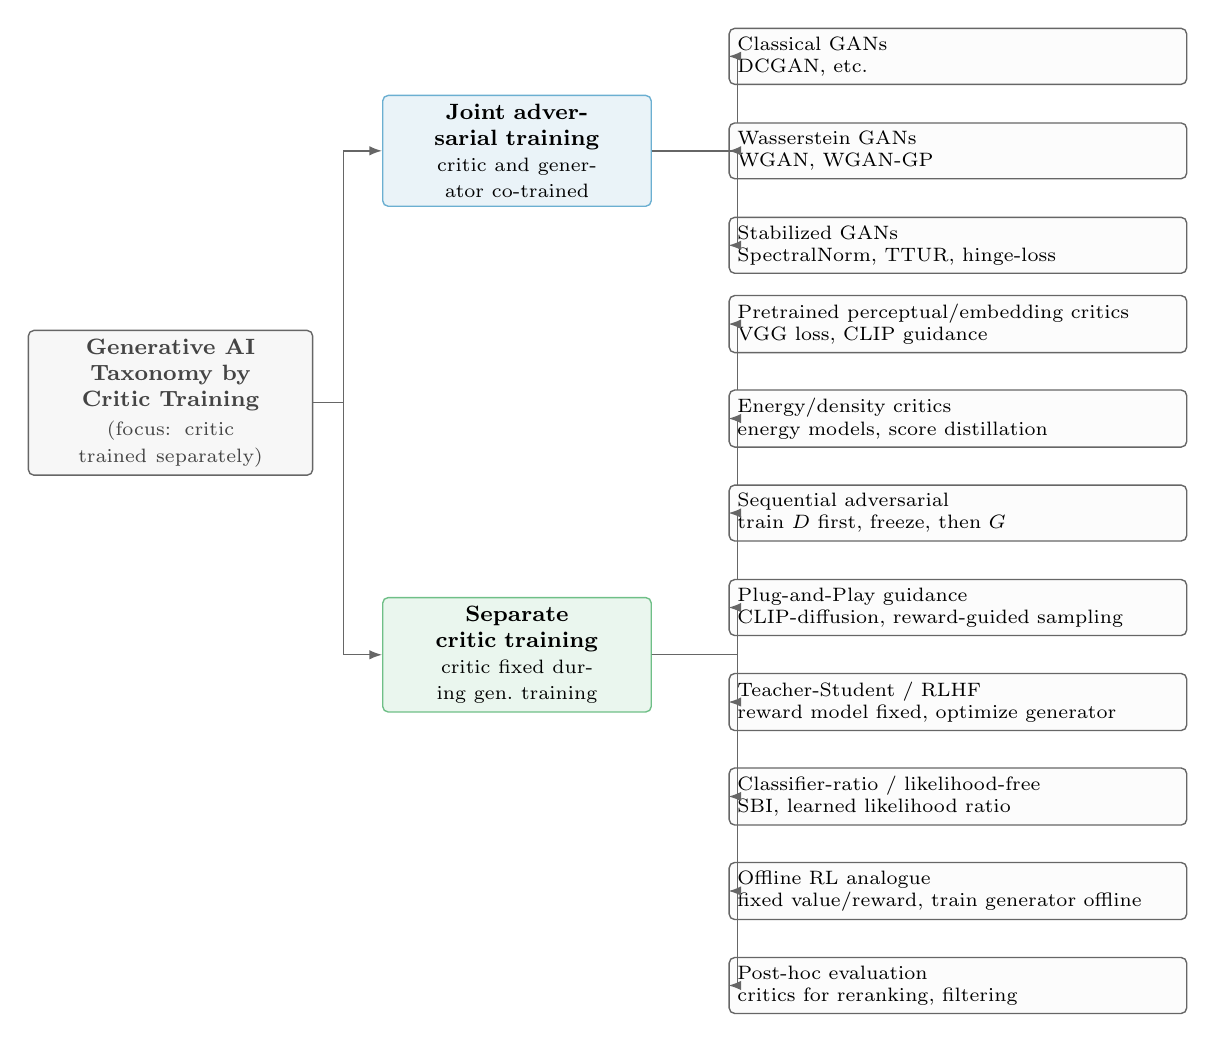
\begin{tikzpicture}[
  grow'=right,
  edge from parent fork right,
  edge from parent/.style={draw=black!60, line width=0.5pt, -{Latex[length=1.6mm]}},
  every node/.style={rounded corners=2pt, draw=black!60, line width=0.5pt, fill=white, inner sep=3pt},
  head/.style={fill=black!3, font=\bfseries\footnotesize, text=cat, align=center, text width=3.4cm},
  branchJ/.style={fill=joint!10, draw=joint!70, align=center, text width=3.2cm, font=\footnotesize},
  branchS/.style={fill=separate!10, draw=separate!70, align=center, text width=3.2cm, font=\footnotesize},
  leaf/.style={fill=black!1, align=left, font=\scriptsize, text width=5.6cm},
  level 1/.style={level distance=4.4cm, sibling distance=6.4cm},
  level 2/.style={level distance=5.6cm, sibling distance=1.2cm}
]
\node[head] {Generative AI Taxonomy by Critic Training\\[1pt] {\scriptsize\mdseries (focus: critic trained separately)}}
  child { node[branchJ] {\textbf{Joint adversarial training}\\ {\scriptsize critic and generator co-trained}}
    child { node[leaf] {Classical GANs\\ {\scriptsize DCGAN, etc.}} }
    child { node[leaf] {Wasserstein GANs\\ {\scriptsize WGAN, WGAN-GP}} }
    child { node[leaf] {Stabilized GANs\\ {\scriptsize SpectralNorm, TTUR, hinge-loss}} }
  }
  child { node[branchS] {\textbf{Separate critic training}\\ {\scriptsize critic fixed during gen.\ training}}
    child { node[leaf] {Pretrained perceptual/embedding critics\\ {\scriptsize VGG loss, CLIP guidance}} }
    child { node[leaf] {Energy/density critics\\ {\scriptsize energy models, score distillation}} }
    child { node[leaf] {Sequential adversarial\\ {\scriptsize train $D$ first, freeze, then $G$}} }
    child { node[leaf] {Plug-and-Play guidance\\ {\scriptsize CLIP-diffusion, reward-guided sampling}} }
    child { node[leaf] {Teacher-Student / RLHF\\ {\scriptsize reward model fixed, optimize generator}} }
    child { node[leaf] {Classifier-ratio / likelihood-free\\ {\scriptsize SBI, learned likelihood ratio}} }
    child { node[leaf] {Offline RL analogue\\ {\scriptsize fixed value/reward, train generator offline}} }
    child { node[leaf] {Post-hoc evaluation\\ {\scriptsize critics for reranking, filtering}} }
  };
\end{tikzpicture}
\end{center}

\paragraph{Plain-English payoff.}
When you start a GAN project, the practical decision tree is short. Use the DCGAN backbone unless you have a reason not to. Train it with WGAN-GP rather than the original JSD loss unless you are deliberately reproducing the classic. If you need control over the output, add a conditioning variable $y$ and you have a Conditional GAN; if you need image-to-image translation, Pix2Pix (paired data) or CycleGAN (unpaired data) is the standard starting point. If you need photorealism at high resolution, that is StyleGAN territory, which is a research-scale compute commitment (Topic 4). And if the adversarial dynamics themselves are the problem, the family tree reminds you that the critic can be trained first and frozen, which trades some flexibility for far more stable optimization.

\paragraph{Further reading.}\begingroup\sloppy
A.\ Radford, L.\ Metz, S.\ Chintala, ``Unsupervised Representation Learning with Deep Convolutional Generative Adversarial Networks,'' ICLR 2016, arXiv:1511.06434. M.\ Mirza, S.\ Osindero, ``Conditional Generative Adversarial Nets,'' 2014, arXiv:1411.1784. P.\ Isola et al., ``Image-to-Image Translation with Conditional Adversarial Networks,'' CVPR 2017. J.-Y.\ Zhu et al., ``Unpaired Image-to-Image Translation using Cycle-Consistent Adversarial Networks,'' ICCV 2017. T.\ Karras, S.\ Laine, T.\ Aila, ``A Style-Based Generator Architecture for Generative Adversarial Networks,'' CVPR 2019. Foster (2023), Chapter 4 (DCGAN) and Chapter 9 (modern variants).
\endgroup

% ======================================================================
\section{Topic 4: Comparing Sample Realism, Controllability, and Training Cost}
% ======================================================================

\paragraph{Plain-English summary.}
GANs are not the only generative-model family, and they are far from the obvious choice for every problem. This topic puts GANs side by side with VAEs (Module 2) along three practical dimensions: \emph{sample realism} (how good do the outputs look?), \emph{controllability} (can you make the model produce a specific kind of output?), and \emph{training cost} (how much compute and how much human attention does it take?). It also previews where diffusion models (Module 5) sit on the same axes, which explains why diffusion has taken over much of the GAN application space.

\subsection{Sample Realism}

A VAE with a Gaussian decoder is trained to maximize
\[
\mathrm{ELBO}(\theta,\phi) = \E_{q_\phi(z\given x)}\big[\log p_\theta(x\given z)\big] - \KL\big(q_\phi(z\given x)\,\|\,p(z)\big),
\]
and with $p_\theta(x\given z)=\mathcal{N}(x;\mu_\theta(z),\sigma^2 I)$ the first term is a per-pixel squared error. The decoder is therefore rewarded for producing the \emph{conditional mean} of all plausible images given $z$, and the mean of a multimodal set of sharp images is a blurry image. GANs have no per-pixel reconstruction term at all; the generator is rewarded only for producing something the discriminator cannot distinguish from real data, which is a statement about the whole distribution, not about pixelwise closeness to any particular training image. This is the headline reason to reach for a GAN: \textbf{sharpness}.

The asterisk is that GAN samples are sharp \emph{in the modes they cover}. A GAN that has dropped modes (Topic 2) produces samples that are sharp and incomplete. A VAE covers the modes (its KL regularizer pushes it toward broad coverage) at the cost of sharpness. The two families fail in opposite directions.

\subsection{Evaluation: The Metrics and What They Do Not Tell You}

Quantifying ``sample quality'' is a research problem in its own right. Two metrics dominate the image literature; both rely on a pretrained Inception classifier as a feature extractor.
\begin{itemize}
    \item \textbf{Fr\'echet Inception Distance (FID)} (Heusel et al., 2017). Pass real and generated samples through the Inception network, take the activations of an intermediate layer, fit a Gaussian $\mathcal{N}(\mu_r,\Sigma_r)$ to the real features and $\mathcal{N}(\mu_g,\Sigma_g)$ to the generated features, and compute
    \[
    \mathrm{FID} = \|\mu_r-\mu_g\|_2^2 + \operatorname{Tr}\!\Big(\Sigma_r+\Sigma_g-2\big(\Sigma_r\Sigma_g\big)^{1/2}\Big).
    \]
    Lower is better. FID is the de facto standard for comparing image GANs and is itself a Wasserstein-2 distance between the two fitted Gaussians, so it is sensitive to both quality and diversity.
    \item \textbf{Inception Score (IS)} (Salimans et al., 2016). Let $p(y\given x)$ be the classifier's label distribution for a sample $x$ and $p(y)=\E_x[p(y\given x)]$ the marginal over generated samples. Then
    \[
    \mathrm{IS} = \exp\Big(\E_{x\sim p_g}\big[\KL\big(p(y\given x)\,\|\,p(y)\big)\big]\Big).
    \]
    Higher is better: it rewards samples that are individually confidently classified (sharp) and collectively spread over many classes (diverse). IS has largely been superseded by FID but is still reported.
\end{itemize}
What these metrics do not tell you is how good the samples are for \emph{your} use case. Both are calibrated on natural-image benchmarks and depend on Inception being a sensible feature extractor for your domain. For medical images, scientific data, audio, or anything outside Inception's training distribution, FID is at best a rough proxy; the appropriate replacement is usually a domain-specific feature extractor plus a downstream-task evaluation, combined with visual inspection.

\subsection{Controllability}

A vanilla GAN has essentially no controllability: you draw $z\sim p_z$ and get whatever the generator produces. Controllability has to be designed in.
\begin{itemize}
    \item \textbf{Conditional GAN}: the conditioning variable $y$ (class label, caption, sketch) is an explicit input, as in \eqref{eq:cgan}.
    \item \textbf{StyleGAN}: the mapping network exposes interpretable style vectors at several resolutions, so coarse attributes (pose, shape) can be edited independently of fine texture.
    \item \textbf{VAE comparison}: a VAE gives you the latent space directly through its encoder $q_\phi(z\given x)$, so you can encode an existing sample, do latent arithmetic, and decode. A vanilla GAN has no encoder; editing a given real image requires a separate inversion step that solves $\argmin_z \|G_\theta(z)-x\|$ or trains an auxiliary encoder.
\end{itemize}

\subsection{Training Cost}

GANs are notoriously expensive to train at quality, and the cost is dominated by human attention as much as by compute:
\begin{itemize}
    \item Foster's \texttt{01\_dcgan} notebook on the LEGO bricks dataset (about 40{,}000 grayscale $64\times 64$ images) is light enough for a laptop or a CPU-only notebook session if you cut the epoch count well below Foster's 300.
    \item The \texttt{02\_wgan\_gp} and \texttt{03\_cgan} notebooks on CelebA (about 200{,}000 RGB faces) want a GPU; expect hours per run on CPU. In these two notebooks an ``epoch'' is only one or two batches by design, so think in training steps rather than epochs.
    \item StyleGAN2 on FFHQ at $1024\times 1024$ takes weeks on multi-GPU clusters, which is not realistic for a course project.
\end{itemize}
WGAN-GP adds a further constant factor: every critic step backpropagates through $\nabla_{\hat x} f_w(\hat x)$, and the critic is updated $n_{\text{critic}}$ times per generator step. If a project requires a high-quality GAN, scope it around what can be trained on the university HPC cluster in a reasonable time.

\subsection{VAE vs.\ GAN vs.\ Diffusion: A Summary Table}

\begin{center}
\renewcommand{\arraystretch}{1.2}
\begin{tabular}{@{}p{2.9cm}p{4.0cm}p{4.0cm}p{4.0cm}@{}}
\toprule
\textbf{Dimension} & \textbf{VAE (Module 2)} & \textbf{GAN (Module 3)} & \textbf{Diffusion (Module 5)} \\
\midrule
Training objective & ELBO, an explicit lower bound on log-likelihood & Minimax / saddle point; no explicit likelihood & Variational bound on likelihood via a denoising objective \\
Encoder & Yes, $q_\phi(z\given x)$ trained with the decoder & None (vanilla); separate inversion step needed & Fixed forward noising process; no learned encoder needed \\
Sample sharpness & Blurry (Gaussian decoder) & Sharp when training succeeds & Sharp, competitive with the best GANs \\
Mode coverage & Broad (KL regularizer) & Can drop modes & Broad (likelihood-based) \\
Training stability & Routine & Hard; four named failure modes & Routine \\
Sampling cost & One decoder pass & One generator pass & Many denoising steps; slow \\
Controllability & Latent arithmetic on the encoded $z$ & Needs Conditional GAN, StyleGAN, etc. & Conditioning and guidance are native \\
Likelihood evaluation & Yes (via ELBO) & No closed form & Yes (bound) \\
Typical use cases & Representation learning, anomaly detection, controllable generation & High-quality image synthesis, image-to-image translation, style transfer & Text-to-image, video, audio; the dominant approach since 2022 \\
\bottomrule
\end{tabular}
\end{center}

\subsection{Where Diffusion Will Fit}

Diffusion models are the most recent answer to the question ``what if we could get GAN-like sharpness without the GAN training difficulty?'' They have an explicit variational training objective like VAEs, produce samples competitive with the best GANs, support conditioning natively, and have been the dominant approach in image, video, and audio generation since 2022. The trade-off is that sampling is slow (many denoising steps) and training requires more compute than a comparable VAE. The Module 5 notes develop this family in full; for now, the point is that the space of choices is wider than VAE versus GAN.

\paragraph{Plain-English payoff.}
The choice among the three families is a choice about which failure you can live with. If you need a latent space you can encode into and reason about, and blur is acceptable, use a VAE. If you need sharp images at modest resolution, can afford a few hours of GPU time and some babysitting of the training run, and can tolerate the risk of dropped modes, use a GAN with the DCGAN backbone and WGAN-GP loss. If you need sharpness and coverage and native conditioning and can afford slow sampling, diffusion is the modern default. Whichever you pick, do not trust FID alone outside natural images; pair it with a domain-appropriate metric and look at the samples.

\paragraph{Further reading.}\begingroup\sloppy
M.\ Heusel et al., ``GANs Trained by a Two Time-Scale Update Rule Converge to a Local Nash Equilibrium,'' NeurIPS 2017, arXiv:1706.08500 (introduces FID). T.\ Salimans et al., ``Improved Techniques for Training GANs,'' NeurIPS 2016, arXiv:1606.03498 (introduces IS). L.\ Theis, A.\ van den Oord, M.\ Bethge, ``A Note on the Evaluation of Generative Models,'' ICLR 2016, arXiv:1511.01844. A.\ Borji, ``Pros and Cons of GAN Evaluation Measures: New Developments,'' CVIU 2022, arXiv:2103.09396. Foster (2023), Chapter 4, section ``Analysis of the WGAN-GP.''
\endgroup

\end{document}
